Our experiments are based on Social Ways. A major change in Social Ways compared to previously implemented GAN models for trajectory prediction is that it implements the InfoGAN architecture. The results from Social Ways~\cite{DBLP:journals/corr/abs-1904-09507} show that InfoGAN can greatly improve the trajectory prediction of multimodal pedestrians, avoiding pattern collapse and degradation. Figure 2 illustrates the architecture.


In the following subsections, we will describe the key methods of Social Ways and our experiments.

\subsection{Methodology}


\subsubsection{Generative Adversarial Networks}
\hfill \\
According to the research of Generative Adversarial Nets~\cite{gan}: a Generative Adversarial Network (GAN) consists of two network components, a discriminator $D$ and a generator $G$, which compete with each other. $G$ takes the input noise variable $z$ and generates the sample $G(z)$, $D$ takes the generated sample or training data as input $x$ and predicts the probability $D(x)$ that $x$ comes from the data and not generated by $G$. $D$ is trained to maximize the probability of assigning correct labels to training samples and generated samples, while $G$ is trained to minimize the correctness of $D$. In other words, $D$ and $G$ play a min-max game with the value function $V(G, D)$.

\begin{multline}
  \min_{G} \max_{D} V(G, D) = \mathbb{E}_{x \sim p_{\text{data}}} \lbrack \log(D(x))\rbrack \\ + \mathbb{E}_{z \sim p_{z}(z)} \lbrack \log(1 - D(G(z))) \rbrack
\end{multline}

In our case, for pedestrian trajectory data, the generator is trained to generate possible future trajectories that have a distribution similar to the training data, given certain previously observed trajectories, while the discriminator learns to distinguish the rationality of the generated paths. These two networks are trained simultaneously. As the discriminators are learned, the generators are improved.

\subsubsection{InfoGAN}

\hfill \\
The algorithm infoGAN bases on Generative Adversarial Network(GAN). Even though Generator of GAN can generate fake examples from the noise input \(\mathbf{z}\), this noise vector is entangled. In other words, we can not deduce any information from the input noise vector and can not control the output of the Generator. What the data the Generator will produce is totally random. Based on GAN, infoGAN is a way that learning interpretable representation by information. It can deduce meaningful information from the input data. Instead of using single noise input, infoGAN accepts another input which is called latent code \(\mathbf{c}\). This latent code can be discrete or continuous. When it is discrete, a integer vector can be used to represent different factors. During training, the vector should be encoded by one hot code. Generator also contains another neural network Q which is called auxiliary network. It takes the fake data that generated by G and output the decoded latent code \( \mathbf{\hat{c}}\). By maximizing the mutual information between \( G(\mathbf{z, c})\) and \( \mathbf{\hat{c}}\), G and Q are trained. The system structure of infoGAN is in \ref{infoGan}. The min-max game of infoGAN is a game with the value function\cite{infogan}:
\[\min_{G,Q}\max_{D} \mathbf{V_{infoGAN}}(D, G, Q) = \mathbf{V}_{D, G} - \lambda \mathcal{L_I}(G,Q),\] where \(\mathcal{L_I}(G,Q)\) is the lower bound of the mutual information \(\mathbf{I}(c;G(z,c))\).
\begin{figure*}[h]
  \centering
  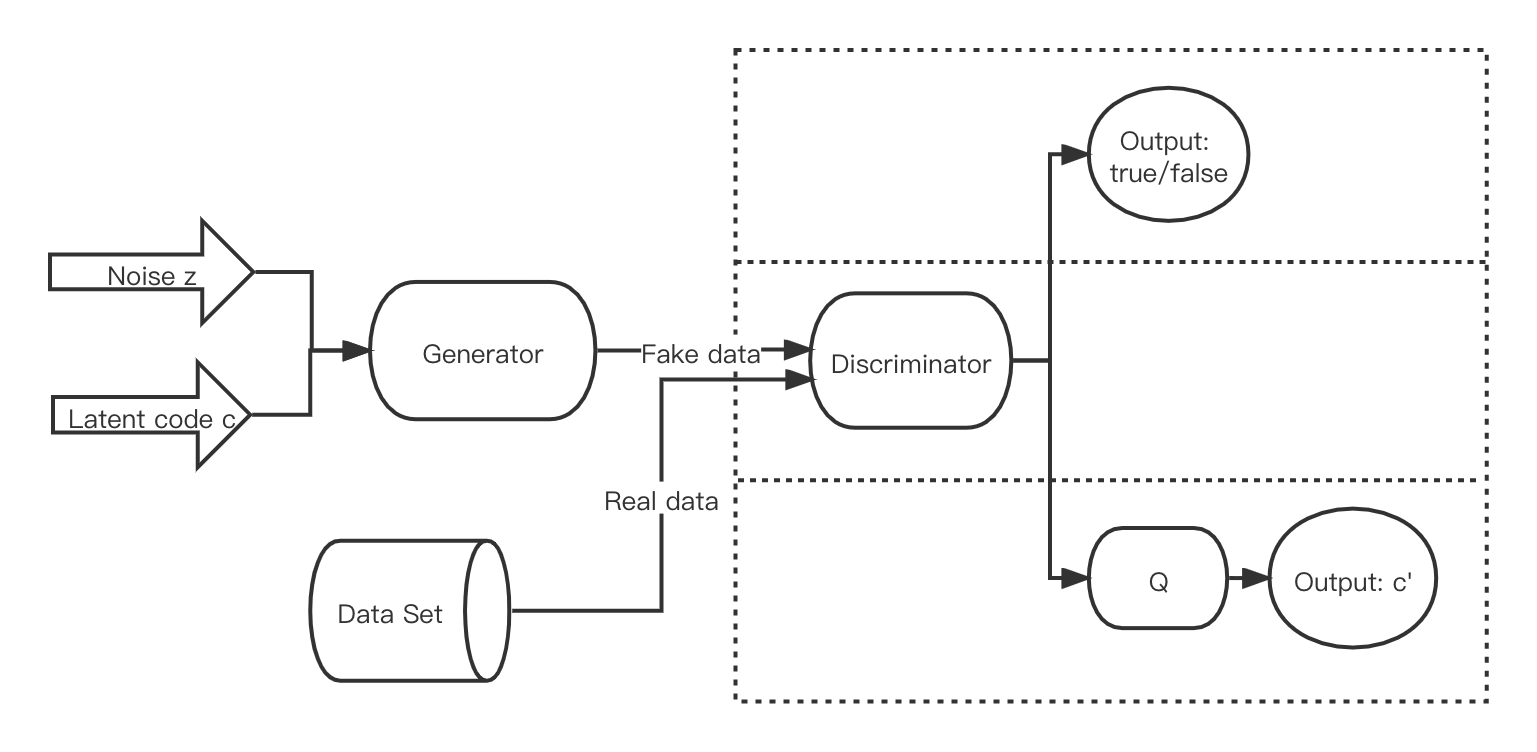
\includegraphics[width=\textwidth, height = 7cm]{figures/infoGAN.png}
  \caption{infoGAN Overview}{infoGAN consists of three parts, Generator G, Discriminator D and auxiliary network Q. D and Q share the network, only their last layers are different.}
%   \Description{infoGAN consists of 3 parts, Generator G, Discriminator D and auxiliary network Q. D and Q share the network, only their last layers are different.}
  \label{infoGan}
\end{figure*}
\subsubsection{Description of Latent Code}

\hfill \\
Our experiments attempt to disentangle the latent code so that the latent code can correspond to the semantic features of the data. To enrich our expression, we allow two types of latent codes, categorical latent codes and continuous latent codes.

For categorical latent code $c$, we can use cross entropy as a loss function to maximize the information between the code and the code predicted by $Q$.


$$\mathcal{L} (c, Q(G(x, c))) = MSE(c, Q(G(x, c))) $$

For a continuous latent code $c$, we can use the mean squared error as a loss function to maximize the information between the code and the code predicted by $Q$.

$$\mathcal{L} (c, Q(G(x, c))) = CE(c, Q(G(x, c))) $$

On the basis of categorical latent codes and continuous latent codes, we can introduce a series of semantic factors. For example, velocity and direction can be represented as continuous latent codes and scenes can be expressed as categorical latent codes. For map/obstacle information, the image embedding of the background image (the background image of the video recording trajectory data) can be used as a sequence of continuous latent codes.

\subsubsection{Experimental Setup}

\hfill \\
In our project, we will train the model using three integer latent codes and three continuous latent codes. At every loop of the training of G, we modify the noise vector as the combination of an one-hot encoded vector with three random integer numbers and another vector with three random float numbers.

After the model is trained, we need to evaluate the latent codes by the method called latent traversal. Assume the discrete codes are \(\mathbf{C_1} = c_1, c_2, c_3\) and the continuous codes are  \(\mathbf{C_2}= c_4, c_5, c_6\). First we fix \(\mathbf{C_2}\) and set \(c_1 = 1, c_2 = 0, c_3=0\), then use the trained G to generate 10 trajectories. Then we draw 10 samples from the generated examples and plot the trajectories as pictures \(Pic_1\). Then fix \(\mathbf{C_2}\) and set \(c_1=0, c_2 = 1, c_3 = 0\) and generate 100 trajectories and take random 10 plot as pictures. We conduct the same process to each integer variables. Then we observe the trajectories in the picture and infer the possible factor that affects the trajectories. Our guess is speed and direction. We can start inferring  from these two factors. If we can find out the pattern in the trajectories, we can match them to the vector of integer latent codes. When evaluate the continuous codes, just fix the other two codes and change the one that is being evaluated by 0.1 every loop, the value of the code value should be in [0.1, 0.3, 0.5, 0.7, 0.9]. There will be \(3 \times 5 = 15\) groups of pictures. We observe the picture and try to deduce the factors from the trajectories.